\documentclass[two column, twoside, a4paper]{article}

\usepackage[utf8]{inputenc}
\usepackage{dblfloatfix}
\usepackage{subcaption}
\usepackage{float}
\usepackage[backend=biber, maxbibnames=3, style=nature, autocite=inline]{biblatex}
\usepackage[polish]{babel}
\usepackage[T1]{fontenc}
\usepackage{fancyhdr}
\usepackage{titlesec}
\usepackage{blindtext}
\usepackage{cuted}
\usepackage{tikz}
\usepackage[most]{tcolorbox}
\usepackage[columnsep = 1cm,
	        lmargin = 0.6in,
	        rmargin = 0.4in,
	        tmargin = 0.5in,
	        bmargin = 0.65in,
	        headsep = \baselineskip]{geometry}

\addbibresource{$BIB}

% Custom commands
\newcommand*\circled[1]{\tikz[baseline=(char.base)]{
            \node[shape=circle,draw,inner sep=2pt, color = orange!90!white] (char) {#1};}}

% Section Formatting
\titleformat{\section}
{\sc \bfseries \Large}
{}
{0em}
{}[\titlerule]

\titleformat{\subsection}
{\bfseries \large}
{}
{0em}
{}

\titleformat{\subsubsection}
{\bfseries}
{}
{0em}
{}

% Box formatting
\tcbset{enhanced, colback=orange!15!white, boxrule = 1pt, coltitle = orange!90!white, colbacktitle = orange!15!white, colframe= orange!50!white}

\pagestyle{fancy}
\fancyhf{}
\fancyhead[RE, LO]{Szkoła Główna Gospodarstwa Wiejskiego}
\fancyhead[LE, RO]{Biotechnologia}
\fancyfoot[RE, LO]{Jakub J. Guzek}
\fancyfoot[LE, RO]{\thepage}
\fancyfoot[CE,CO]{Zmiany w organizmie matki i dziecka w czasie ciąży, hormonalna regulacja porodu}
\renewcommand{\footrulewidth}{0.05pt}

\begin{document}

\begin{strip}
{\sc \bfseries \LARGE \fontfamily{phv}\selectfont Zmiany w organizmie matki i dziecka w czasie ciąży,

\vspace{2pt} hormonalna regulacja porodu} \vspace{\baselineskip}

{\bfseries \large Jakub J. Guzek}

{Szkoła Główna Gospodarstwa Wiejskiego, Biotechnologia, Nr. albumu: 195528}\vspace{\baselineskip}

\hrule
\end{strip}

\section{Wstęp}

Ciąża, poród, a także inne procesy związane z rozrodem u ssaków są kontrolowane przez skomplikowany system, w którym ściśle współpracuje ze sobą wiele hormonów i substancji regulujących, przy jednoczesnej współpracy układu nerwowego. Taka regulacja neurohormonalna działająca na wielu poziomach, umożliwia dokładną kontrolę skomplikowanych procesów rozwojowych zachodzących w rozwijającym się zarodku oraz interakcję między procesami zachodzącymi w organizmie matki i dziecka. Wiele z substancji biorących udział w tej regulacji wykazuje działanie wielotorowe na wiele różnych tkanek zarówno u matki, jak i u dziecka i dodatkowo obecne są znaczne różnice w ich działaniu między gatunkami.
Z tego powodu omówienie działania poszczególnych hormonów oddzielnie, zaciera istotę interakcji jakie zachodzą w tych procesach na wielu poziomach -- znacznie korzystniejsze jest omówienie działania tych substancji w ujęciu systemicznym, jako dynamicznego biologicznego systemu, którego struktura ulega znacznym zmianom w czasie. Omówienie jednak tego zagadnienia w ujęciu biologii systemów jest skomplikowane -- należy bowiem pamiętać, że sieć interakcji między hormonami i ich receptorami w czasie ciąży i porodu nie jest odizolowana od innych tego rodzaju sieci w reszcie organizmu oraz że wiele interakcji w takim układzie ma charakter zmienny nie tyko w zależności od czasu ale także od czynników środowiskowych.

\begin{figure}[t]
\begin{tcolorbox}[title=\hspace{-1.5em} \circled{\textbf{Box 1}} \textbf{\large{Wyjaśnienie skrótów}}]
	\begin{description}
		\item[ACTH] -- hormon adenokortykotropowy (\textit{ang, adrenocorticotropic hormone})
		\item[AMH] -- \textit{anti-M\"{u}llerian hormone}
		\item[CRH] -- kortykoliberyna (\textit{ang. corticotropin-realising hormone})
		\item[DHT] -- dihydroksytestosteron
		\item[eCG] -- końska gonadotropina kosmówkowa (\textit{equine chorion gonadotropin})
		\item[ER] -- retikulum endoplazmatyczne
		\item[FSH] -- hormon folikulotropowy (\textit{ang. follicle-stimulating hormone})
		\item[GH] -- hormon wzrostu (\textit{ang. growth hormone})
		\item[GnRH] -- gonadoliberyna (\textit{ang. gonadotropin-releasing hormone})
		\item[hCG] -- ludzka gonadotropina kosmówkowa (\textit{ang. human chorion gonadotropin})
		\item[LEP] -- leptyna (\textit{ang leptin})
		\item[LH] -- hormon luteinizujący (\textit{ang. luteinizing hormone})
		\item[OX] -- oksytocyna (\textit{ang. oxytocin})
		\item[PG] -- prostaglandyny
		\item[PRL] -- prolaktyna (\textit{ang. prolactin})
	\end{description}
\end{tcolorbox}
\end{figure}

\section{Przed ciążą}

Oogeneza rozpoczyna się u samic wielu gatunków ssaków już na etapie życia płodowego. Pierwotne komórki płciowe są po migracji do zawiązków gonad przekształcane w oogonia. Oogonia ulegają w dalszej kolejności wielu podziałom mitotycznym po których rozpoczyna się podział mejotyczny, który ulega zatrzymaniu na etapie profazy mejozy I -- komórka taka nazywa się oocytem I rzędu i może pozostawać w takim stadium przez długi czas aż samica osiągnie dojrzałość płciową. \autocite{Krzymowski2005}

Po osiągnięciu przez samicę dojrzałości płciowej oocyty rosnących pęcherzyków jajnikowych przechodzą dalsze etapy podziału mejotycznego aż do ponownego zatrzymania procesu na etapie metafazy mejozy II \autocite{Sawicki2017}. Dojrzewanie pęcherzyków jajnikowych zachodzi cyklicznie od kiedy samica osiągnie dojrzałość płciową.

 \begin{figure*}[bp]
	 \begin{tcolorbox}
		 \centering
		 \begin{subfigure}[b]{0.4\textwidth}
			 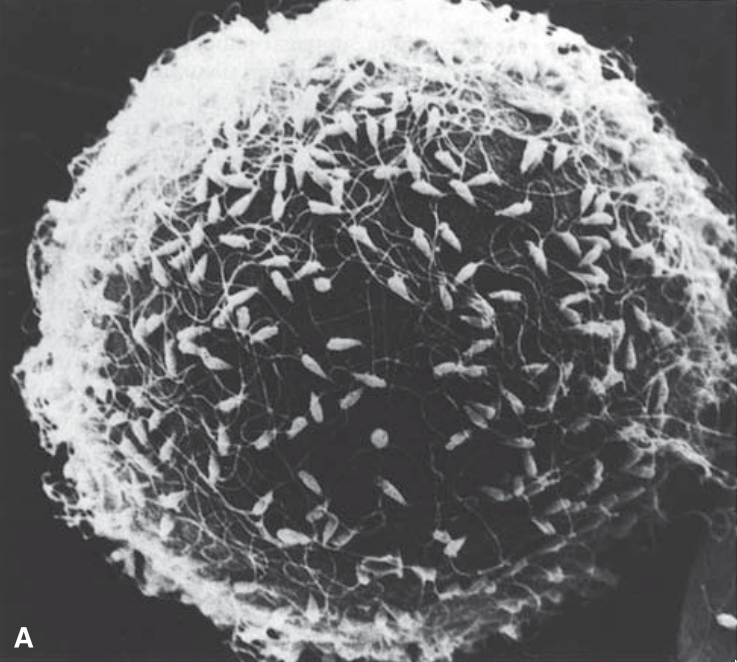
\includegraphics[width=\textwidth]{./figures/fertilization.png}
		\caption{}\label{fig::fertilization:a}
		\end{subfigure}
		 \begin{subfigure}[b]{0.5925\textwidth}
			 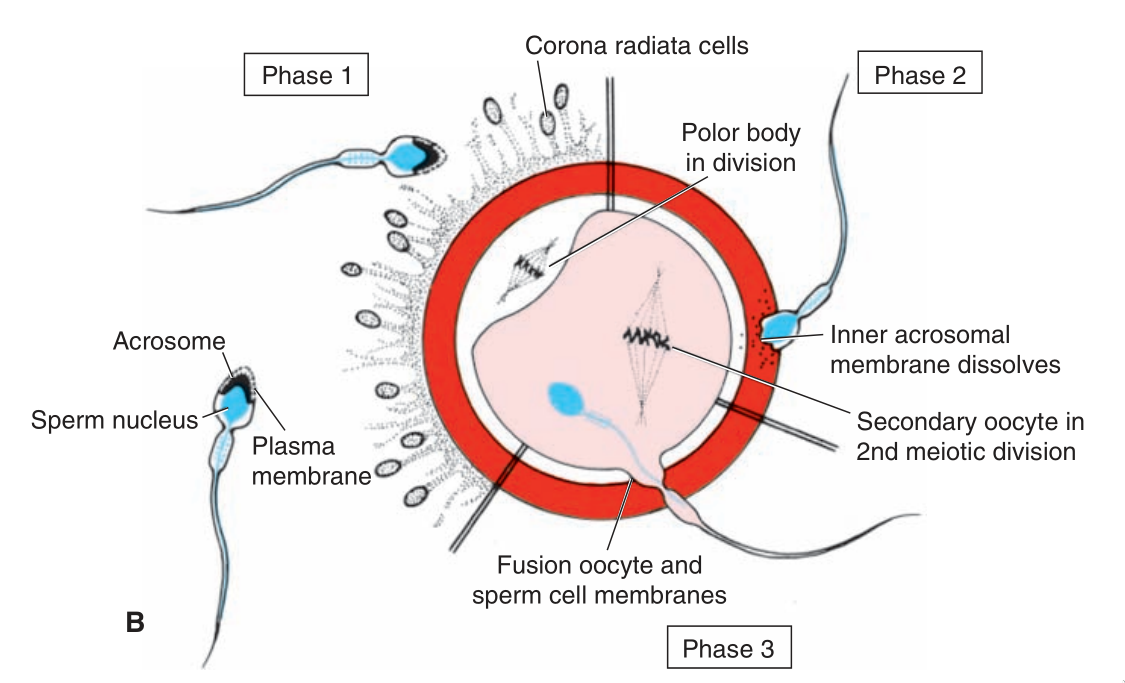
\includegraphics[width=\textwidth]{./figures/fertilization2.png}
		\caption{}\label{fig::fertilization:b}
		\end{subfigure}
		 \caption{(a) Fotografia ze skaningowego mikroskopu elektronowego przedstawiająca plemniki wiążące się do osłonki przejrzystej oocytu. (b) Trzy fazy penetracji oocytu. W fazie pierwszej plemniki przedostają się przez wieniec promienisty; w fazie drugiej jeden lub więcej plemników przedostają się przez otoczkę przejrzystą. W fazie trzeciej jeden plemnik dostaje się do oocytu, tracąc przy tym własną plazmolemę. Na podstawie (Sadler, 2012)}\label{fig::fertilization}
	\end{tcolorbox}
\end{figure*}

\subsection{Regulacja czynności jajnika i dojrzewania pęcherzyków jajnikowych}

Najwięcej pęcherzyków jajnikowych występuje jako pierwotne pęcherzyki jajnikowe -- pozostają one w tym stadium przez kilka do kilkunastu lat (w zależności od gatunku). Niektóre z pęcherzyków pierwotnych ulegają przekształceniu w pęcherzyki rosnące, pęcherzyki antralne i na koniec w pęchrzyki przed owulacyjne. Ważną rolę w dalszych etapach dojrzewania pęcherzyków (po wykształceniu przez pęcherzyk otoczki przejrzystej, wieńca promienistego, błony ziarnistej oraz otoczek zewnętrznej i wewnętrznej) odgrywają komórki osłonki wewnętrznej i błony ziarnistej (tzw. komórki ziarniste). Wykształcają one na swojej powierzchni receptory hormonów gonadotropowych (tj. LH i LSH). Receptory te umożliwiają tym komórkom reakcje na hormony gonadotropowe, która polega na rozpoczęciu przez komórki jajnika syntezy hormonów steroidowych. \autocite{Krzymowski2005}

Pod wpływem hormonu luteinizującego komórki osłonki wewnętrznej wytwarzają adrogeny (androstedion i testosteron). Hormony adrogenne przenikają następnie przez błonę podstawią pęcherzyka jajnikowego do błony ziarnistej, w której pod wpływem FSH aktywowany jest enzymatyczny kompleks aromatazy \autocite{Erickson1978}. Kompleks ten katalizuje przemianę testosteronu do 17$\beta$-estradiolu, który następnie wydzielany jest do naczyń włosowatych, skąd przedostaje się do krwi żylnej \autocite{Abubakar1971}. 17$\beta$-estradiol jest hormonem wydzielanym przez dojrzałe pęcherzyki jajnikowe, i jego wysoki poziom w osłonce wewnętrznej jest dobrym wymiernikiem dojrzałości danego pęcherzyka \autocite{Thorneycroft1971}, przynajmniej w wypadku pęcherzyków jajnikowych kobiet. Stężenie estradiolu jest najwyższe tuż przed owulacją -- rośnie ono przez cały okres dojrzewania pęcherzyka w miarę jego rozwoju. Hormon ten wykazuje hamujące działanie na receptory LH w komórkach ziarnistych -- na zasadzie ujemnego sprzężenia zwrotnego wysokie stężenie estradiolu doprowadza więc do hamowania syntezy testosteronu z cholesterolu przez te komórki.

Ta krótka, parakrynowa pętla regulacyjna czynności jajnika przez wzrastające stężenie estrogenów nie jest jedynym takim mechanizmem. Komórki ziarniste są zdolne do wytwarzania peptydowych związków, o wzajemnie antagonistycznym działaniu -- inhibiny i aktywiny. Inhibina dostaje się z krwią do przysadki mózgowej, gdzie hamuje uwalnianie FSH. Ma to ujemny wpływ na wydzielanie hormonów przez komórki ziarniste. \autocite{Krzymowski2005, Woodruff1995, Findlay1993}

W dojrzewającym pęcherzyku są również obecne inne hormony steroidowe wydzielane przez komórki ziarniste. Są to m. in. progesteron i estron, które stanowią produkty pośrednie w syntezie 17$\beta$-estradiolu z cholesterolu.

Prócz wymienionych wyżej hormonów steroidowych na reglację czynności jajnika i dojrzewania pęcherzyków jajnikowych ma także wpływ wiele innych substancji działających para- i autokrynowo w obrębie tych struktur, a także wiele substancji peptydowych takich jak czynniki wzrostu (IGF-I, IGF-II), czynniki martwicy nowotworów, interferony i interleukiny (IL-1, IL-2, IL-6, IL-8). IGF-I i IGF-II wpływają na proliferację i różnicowanie oraz steroidogenezę w komórkach oraz biorą udział w regulacji angiogenezy pęcherzyka jajnikowego i tworzącego się po jego pęknięciu ciałka żółtego. \autocite{Krzymowski2005, Erickson1990, Gottshall1987, Alpizar1994}

\subsection{Owulacja}

W czasie owulacji dojrzałe pęcherzyki jajnikowe pękają. W tym czasie z pękniętego pęcherzyka uwalniana do jamy brzusznej jest komórka jajowa, która przechwytywana jest przez kosmki jajowodu i wprowadzana jest do jego światła \autocite{Sawicki2017}.

Proces owulacji bezpośrednio poprzedza wydzielanie GmRH, które stymuluje gwałtowny, i długotrwały (trwający ok. kilka do kilkunastu godzin) wyrzut LH z przedniego płata przysadki do krwi. Wysokie stężenie LH w krwiobiegu powoduje unieczynnienie znajdującego się w jamie pęcherzyka jajnikowego inhibitora dojrzewania pęcherzyka. W tym samym czasie we krwi wzrasta również stężenie FSH i PRL. FSH indukuje wytwarzanie w komórkach ziarnistych receptorów dla LH, a LH z pomocą PRL po połączeniu z tymi receptorami rozpoczyna proces luteinizacji tych komórek. Jednocześnie zlokalizowane z jajniku komórki układu odpornościowego wydzielają histaminę co prowadzi do rozszerzenia naczyń krwionośnych doprowadzających krew do pęcherzyka. Wysokie stężenie FSH i LH prowadzi do uczynnienia plazminogenu do plazminy, która następnie wraz z aktywowaną przez progesteron, PGF$_{2\alpha}$ i PGE$_{2}$ kolagenazą rozluźniają połączenia między tworzącymi zrąb otoczki fibroblastami. Na skutek tego następuje osłabienie struktury otoczki zewnętrznej i wewnętrznej pęcherzyka jajnikowego, co prowadzi do jego pęknięcia i uwolnienia komórki jajowej \autocite{Krzymowski2005,Sawicki2017}

Do całego tego procesu dochodzi na skutek dodatniego sprzężenia zwrotnego między estrogenami a wydzielaniem LH, FSG i PRL. Jak wspomniano wcześniej stężenie estrogenóœ (zwłaszcza 17$\beta$-estradiolu) we krwi rośnie wraz dojrzewaniem pęchrzyków jajnikowych i w pewnym momencie doprowadza do wylewu LH do krwi, rozpoczynając wyżej opisane zmiany hormonalne i biochemiczne prowadzące do owulacji.

W kontroli mechanizmu pękania dojrzałego pęcherzyka jajnikowego biorą również udział interleukiny (zwłaszcza IL-1$\beta$), która pobudza syntezę PGE$_{2}$ i PGF$_{2\alpha}$ oraz uwalnianie tlenku azotu. Na syntezę prostaglandyn ma też wpływ czynnik martwicy nowotworów $\alpha$ (TNF-$\alpha$). Co interesujące cytokiny te wykazują podobne działanie u innych grup kręgowców np. ryb doskonałokostnych \autocite{Watanabe1994, Crespo2015, Brannstrom1994, Brannstrom1995}.

\subsection{Regulacja powstawania, zanikania i utrzymywania ciałka żółtego}

Po owulacji pęknięty pęcherzyk jajnikowy wypełnia się skrzepliną, wgłąb której zaczynają wnikać drobne naczynia krwionośne. Rozwój tych naczyń jest ułatwiony przez zanik błony podstawnej nabłonka pęcherzyka. W tym samym czasie we krwi dalej utrzymuje się wysokie stężenie LH, które jak wspomniano już stymuluje luteinizację komórek ziarnistych i komórek osłonki wewnętrznej. U niektórych gatunków(np. świni, szczura i chomika) działanie luteinizujące wykazuje nie tylko LH ale także PRL. Komórki ziarniste ulegają przekształceniu do dużych komórek luteinowych (lub po prostu komórek luteinowych), a komórki osłonki wewnętrznej do małych komórek luteinowych (lub inaczej paraluteinowych) \autocite{Krzymowski2005, Sawicki2017, Greenwald1973}

Luteinizacja tych komórek i wykształcenie się ciałka żółtego z pęcherzyka jajnikowego ma duże znaczenie dla właściwej regulacji hormonalnej w pierwszych etapach ciąży i jej utrzymania. Komórki luteinowe mają na swojej powierzchni wiele receptorów dla LH i wydzielają bardzo wiele hormonów. Pojedyncza komórka luteinowa wydziela więcej progesteronu niż komórka paraluteinowa ale tych drugich jest znacznie więcej dlatego też one są głównymi producentami tego hormonu. Dodatkowo komórki duże prócz progesteronu wydzielają wiele innych hormonów takich jak: oksytocyna, wazopresyna i relaksyna. Mają one receptory dla PGF$_{2\alpha}$ i PGE$_{2}$. U przeżuwaczy komórki te w czasie fazy ciałka żółtego dostarczają do krwiobiegu więcej OX niż podwzgórze. Komórki luteinowe ciałka żółtego zawierają więcej mRNA oksytocyny niż komórki podwzgórza. U większości innych ssaków zawartość tego mRNA w ciałku żółtym jest wielokrotnie niższa \autocite{Krzymowski2005, Jones1988, Ivell1984}.

U większości ssaków ciałko żółte jest jedynym miejscem syntezy relaksyny.

W wypadku braku ciąży ciałko żółte ulega relatywnie szybkiemu zanikowi. Jego utrzymanie jest zależne od stężenia gonadotropin we krwi, które pobudzają to ciałko do wydzielania. Również wydzielany przez samo ciałko żółte progesteron pobudza komórki luteinowe do wydzielania na drodze autokrynowej. Proces zanikania ciałka żółtego zwany luteolizą jest skomplikowany i nie będzie tutaj omówiony.
W ciałku żółtym oprócz komórek luteinowych znajdują się też komórki układu immunologicznego i tkanki łącznej, a także komórki śródbłonka budujące naczynia włosowate \autocite{Krzymowski2005, Sawicki2017}.

\subsection{Zapłodnienie}

Hormony sterujące dojrzewaniem pęcherzyków jajnikowych, owulacją i powstawaniem oraz zanikaniem ciałka żółtego biorą także udział w regulacji cyklu rujowego u większości ssaków i cyklu menstruacyjnego u naczelnych. W fazie owulacyjnej tych cykli oocyt II-rzędu jest wydzielany z pęchrzyków i łapany do światła jajowodu, a następnie ulega tam przemieszczeniu w kierunku macicy i zatrzymaniu na $1/3$ długości górnego odcinka jajowodu, gdzie czeka na zapłodnienie. Oocyt jednak szybko się starzeje i po kilku lub kilkunastu godzinach (w zależności od gatunku) jest niezdolny do zapłodnienia\footnote{w skrajnym wypadku -- u suki oocyt może być zdolny do zapłodnienia przez nawet 5 dni}. Transport komórki jajowej wzdłuż jajowodu jest możliwy dzięki skurczom ścian jajowodu i działaniu rzęsek pokrywających nabłonek tego narządu. Jest to regulowane przez wysoki poziom hormonów jajnikowych (estrogenów i OX) oraz LH i PGF$_{2\alpha}$. \autocite{Krzymowski2005}

Zaplemnienie i zapłodnienie jest złożonym procesem, w którym na skutek kopulacji plemniki są dostarczane do jajowodu gdzie odnajdują komórkę jajową. Przechodzą one po drodze selekcję i kapacytację w skutek czego zmienia się ich morfologia i fizjologia (zwłaszcza akrosomu plemnika). Dokładny przebieg tego procesu nie będzie omówiony.

Plemnik po wniknięciu do oocytu zmienia jego fizjologię -- powoduje aktywację oocytu przez indukcje uwolnienia jonów Ca$^{2+}$ z ER oocytu, oraz uruchomienie bloku przeciwko polispermii (Rysunek \ref{fig::fertilization:a}). Dokończona zostaje w tym czasie mejoza oocytu, wydzielone zostaje ciałko kierunkowe II i powstaje przedjądrze żeńskie. Dochodzi do wymieszania materiału genetycznego pochodzącego od samca i samicy w procesie zwanym kariogamią (Rysunek \ref{fig::fertilization:b}). Zostaje przywrócona diploidalna ilość chromosomów i rozpoczynany jest pierwszy podział mitotyczny nowego organizmu -- zygoty \autocite{Krzymowski2005, Bielanska2001}.

\section{Ciąża}

Opisane w poprzedniej sekcji zmiany hormonalne zachodzące w czasie cykli rozwoju pęcherzyków jajnikowych mają wpływ nie tylko na funkcjonowanie jajników, ale także na inne narządy rozrodcze, całą resztę organizmu, rosnący zarodek a także na zachowanie samicy. Wzrastający we krwi poziom estrogenów (zwłaszcza 17$\beta$-estradiolu) prowadzi do rozrostu błony śluzowej macicy w przygotowaniu na implantację zarodka. Dochodzi do rozrzedzenia śluzu w szyjce macicy w celu ułatwienia przepływu plemników. \autocite{Sawicki2017, Sadler2012}

 \begin{figure}[tp]
	 \begin{tcolorbox}
		 \centering
		 \begin{subfigure}[b]{0.51\textwidth}
			 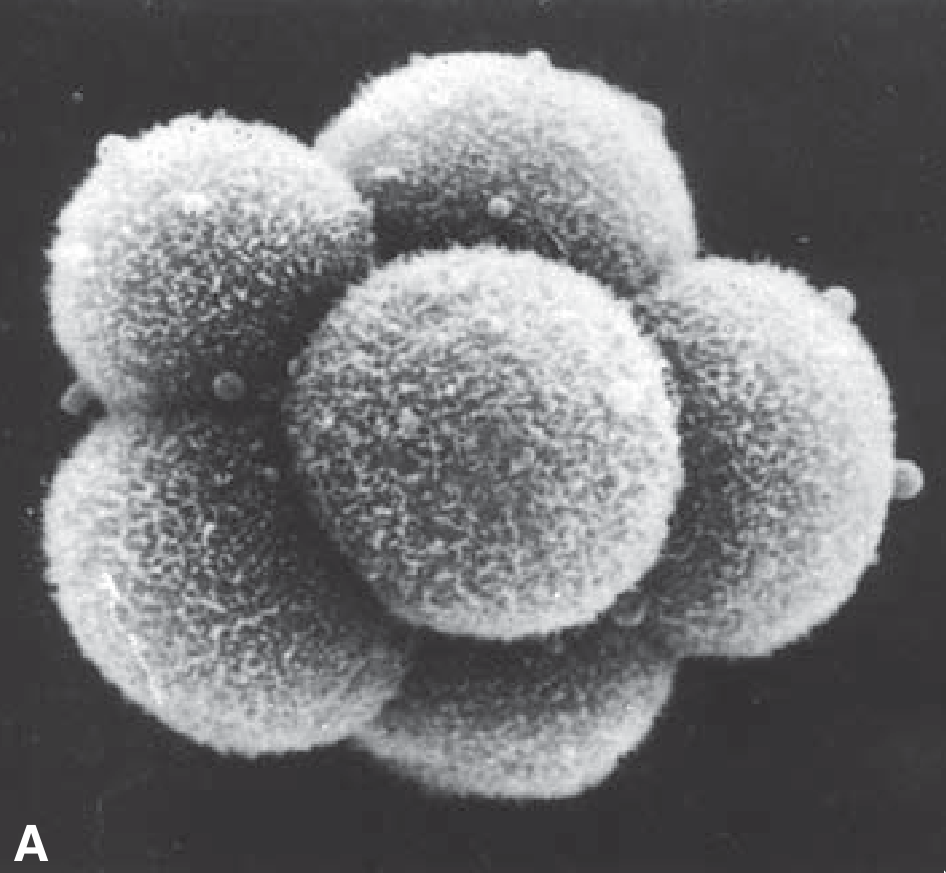
\includegraphics[width=\textwidth]{./figures/blastomeres.png}
		\caption{Wczesna morula (nieskompaktowana)}\label{fig::blastomeres:a}
		\end{subfigure}
		 \begin{subfigure}[b]{0.4755\textwidth}
			 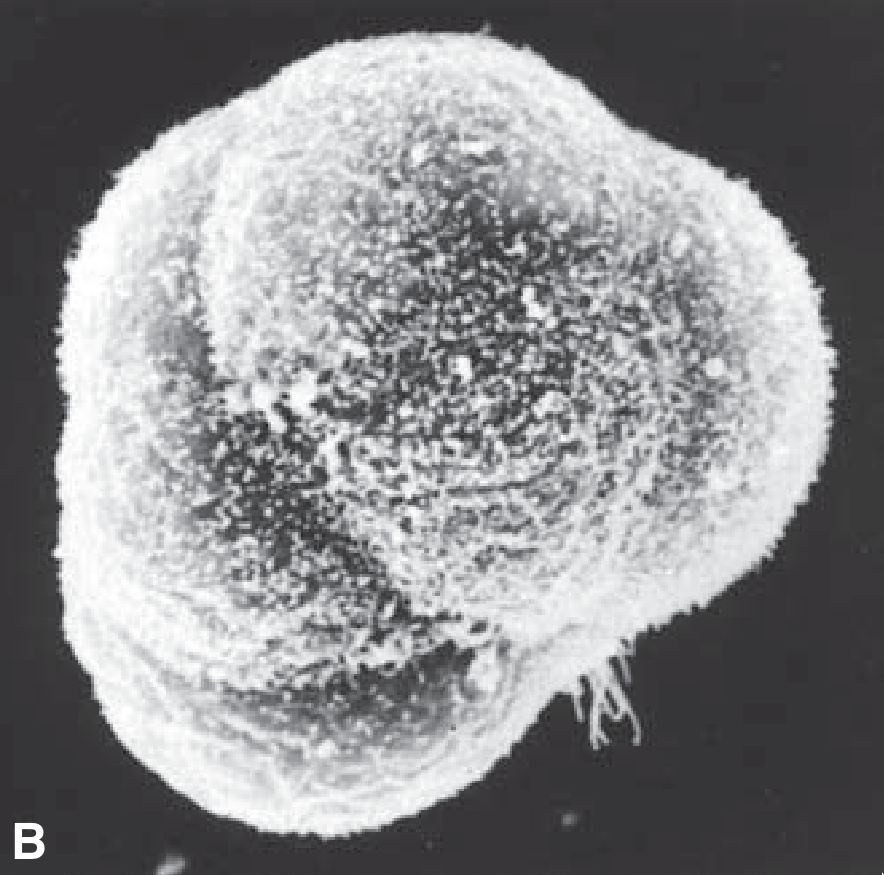
\includegraphics[width=\textwidth]{./figures/blastomeres2.png}
			 \caption{Późna morula (skompaktowana)}\label{fig::blastomeres:b}
		\end{subfigure}
		 \caption{Zdjęcia ze skaningowego mikroskopu elektronowego przedstawiające morulę mysich zarodków w (a) nieskompaktowanym i (b) skompaktowanym stanie. Na podstawie: (Sadler, 2012)}\label{fig::blastomeres}
	\end{tcolorbox}
\end{figure}

 \begin{figure*}[ht!]
	 \begin{tcolorbox}
		 \centering
		 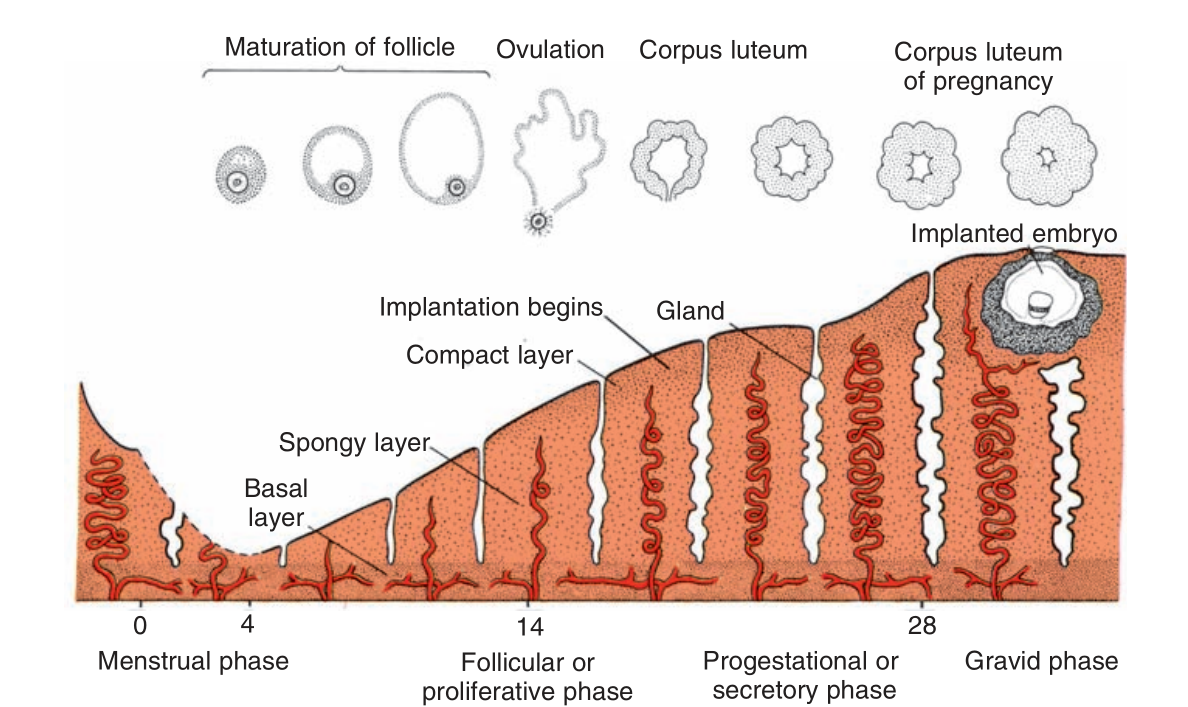
\includegraphics[width=\textwidth]{./figures/endometrium.png}
		 \caption{Zmiany w błonie śluzowej macicy powiązane ze zmianami w pęcherzyku jajnikowym. Implantacja blastocysty sama w sobie nie jest konieczna do utrzymania ciałka żółtego \autocite{Krzymowski2005}, ale związane z nią zmiany w strukturze błony śluzowej macicy i w wydzielaniu indukują przekształcenie ciałka żółtego w ciałko żółte ciążowe. Aktywność wydzielnicza endometrium rośnie w czasie wraz z ilością wydzielanego przez ciałko ciążowe progesteronu. Na podstawie (Sadler, 2012)}\label{fig::endometrium}
	\end{tcolorbox}
\end{figure*}

\subsection{Wczesna ciąża}

Po zakończeniu pierwszego podziału mitotycznego zygoty, przechodzi ona w serie kolejnych takich podziałów w relatywnie krótkim czasie zwiększając liczbę komórek. Komórki te, zwane blastomerami z każdym kolejnym podziałem są coraz mniejsze, gdyż rozmiar całego zarodka pozostaje w tym czasie mniej więcej niezmienny (Rysunek \ref{fig::blastomeres}).

Regulacja procesów kontrolujących właściwy podział blastomerów nie jest do końca poznana, nie ulega jednak wątpliwości, że proces ten musi podlegać ścisłej kontroli, gdyż blastomery wykazują specyficzne wzorce podziałów w czasie bruzdkowania (różne u różnych gatunków). Proponowana była obecność inhibitora interakcji miedzy E-kadherynami i kateninami, który brałby udział w prawidłowym kształtowaniu połączeń między blastomerami i uniemożliwiał przedwczesne przekształcenie moruli w blastulę. Nie ulega wątpliwości że udział w regulacji wczesnych procesów rozwojowych zarodka przed implantacją biorą IGF-I i IGF-II, gdyż są one obecne w dużych ilościach w środowisku rozwoju zarodka. Także matczyne cytokiny wykazują działanie parakrynowe na rozwój zarodka w czasie bruzdkowania. Molekularny mechanizm działania tej regulacji nie jest jednak poznany \autocite{Sadler2012, Bielanska2001, Watson2004}

Stadium przed-implantacyjne trwa od kilku (u gryzoni) do kilkudziesięciu dni (u koni). Samą implantację można podzielić na trzy etapy: etap apozycji, etap adhezji do błony śluzowej macicy i etap inwazji. W fazie apozycji zarodek (w postaci blastocysty u większości ssaków) zajmuje właściwe miejsce w macicy. Zajęcie przez niego tego miejsca jest możliwie dzięki czynnikom chemotaktycznym wydzielanym przez nabłonek śluzowy macicy. Czynnikami tymi są m. in. IL-8 oraz białko chemotaktyczne monocytu 1. Adhezja polega na przylgnięciu zarodka do komórek endometrium przy czym kluczową rolę odgrywają IL-1$\alpha$ i IL-1$\beta$, produkowane przez zarodek. Regulują one ekspresję jednej z podjednostek kompleksu integryn, czyli białek odpowiadający za adhezję komórek. W fazie inwazji zarodek zagłębia się w błonie śluzowej macicy. Umożliwia to działanie enzymów proteolitycznych, w których aktywacji uczestniczą interleukiny (IL-1$\alpha$, IL-1$\beta$, IL-6), czynnik wzrostowy nabłonka (EGF) oraz wspomniane wcześniej integryny. W kontroli całego procesu implantacji uczestniczą także inne hormony -- estrogeny i progesteron, a nawet prolaktyna czy kalcytonina oraz wytwarzana przez zarodek gonadotropina kosmówkowa\footnote{tylko u naczelnych}. Na sam koniec implantacji ważną rolę pełni także VEGF -- czynnik wzrostowy komórek śródbłonka naczyń, który przygotowuje naczynia krwionośne w miejscy implantacji do wytworzenia później łożyska \autocite{Krzymowski2005, Sadler2012, Bielanska2001, Kodaman2004}.

Po implantacji zarodka w błonie śluzowej macicy układ odpornościowy matki ulega wyciszeniu, co zapobiega atakowi immunologicznemu z jego strony na odmienny genetycznie zarodek. Za mechanizm tej immunosupresji odpowiada m. in. progesteron.

Progesteron jest najważniejszym hormonem ciążowym, oprócz immunosupresyjnego działania na organizm matki, odpowiada on za utrzymanie ciąży. We wczesnych fazach ciąży u wszystkich gatunków zwierząt głównym źródłem progesteronu jest ciałko żółte, którego funkcjonowanie zostało omówione wcześniej. U niektórych gatunków zadanie wydzielania progesteronu zostaje szybko przejęte przez łożysko, ale u innych niezakłócone funkcjonowanie ciałka żółtego jest konieczne przez całą ciążę \autocite{Krzymowski2005, Graham1997}.

Zarodki intensywnie wydzielają do środowiska wiele hormonów i substancji regulatorowych, które w znaczący sposób zmieniają funkcjonowanie macicy i innych organów matki, a nawet wpływają na jej zachowanie \autocite{Noirot1975, Rosenblatt1988}. Wytwarzane przez zarodek estrogeny i prostaglandyny (PGF$_{2\alpha}$, PGE$_{2}$. PGI$_{2}$) w pewnym stopniu przenikają do matczynego krwiobiegu, zwiększając ukrwienie macicy.

Wydzielany przez zarodek hormon białkowy przypominający PRL i GH, zwany laktogenem jest kolejną substancją przygotowującą błonę śluzową macicy do implantacji. Bierze on także udział w regulacji angiogenezy w endometrium, a później w łożysku \autocite{Corbacho2002}.

Mimo działania w tych procesach tak wielu hormonów i faktu, że za utrzymanie ciąży odpowiada w pierwszych jej fazach głównie syntezowany przez komórki luteinowe i paraluteinowe progesteron --- przyjmuje się, że sygnałem płodowym odpowiedzialnym za rozpoznanie przez organizm matki ciąży są wytwarzane przez zarodek estrogeny. Hormony te po przeniknięciu do błony śluzowej macicy powodują zmianę kierunku wydzielania PGF$_{2\alpha}$ -- substancja ta przestaje być wydzielana do światła naczyń krwionośnych a zaczyna być wydzialana do światła macicy. Brak tej prostaglandyny we krwi uniemożliwia jej dotarcie do ciałka żółtego, co powstrzymuje proces luteolizy. Jest to główny znany mechanizm hamowania zaniku ciałka żółtego. Inne mechanizmy nie są poznane chociaż pojawiały się badania sugerujące udział hCG w tym procesie\footnote{u kobiet}. który polegałby na regulacji ekspresji genów odpowiedzialnych za luteolizę \autocite{Krzymowski2005, Dickinson2008}.

Taka ścisła interakcja między substancjami regulatorowymi wydzielanymi przez matkę i przez zarodek, umożliwia utrzymanie prawidłowego przebiegu wczesnych faz ciąży. Widać to szczególnie w wypadku rozwoju ciałka żółtego i mechanizmów wpływających na jego utrzymanie i równoczesnych przemianach struktury błony śluzowej macicy (Rysunek \ref{fig::endometrium}).

\subsection{Błony płodowe i łożysko}

W czasie gdy zarodek przechodzi w rozwoju do etapu blastocysty, jego komórki można podzielić na dwie grupy -- komórki tworzące wewnętrzną masę w jamie blastuli nazywa się embrioblastem, a te na zewnątrz, tworzące ,,otoczkę'' blastocelu, nazywa się trofoblastem. Nazwy te nie są przypadkowe gdyż komórki embrioblastu w przyszłości wytworzą właściwy embrion, a komórki trofoblastu wytworzą struktury pełniące wobec embrionu funkcje pomocnicze i odżywcze (\textit{gr. troph\={e}} -- odżywczy, odżywiający), takie jak błony płodowe i łożysko \autocite{Sadler2012, Bielanska2001}

Zadaniem błon płodowych jest zapewnienie łączności między zarodkiem a matką, stworzenie odpowiednich warunków do rozwoju zarodka a później płodu oraz ochrona zarodka. Na pierwszych etapach ciąży trofoblast rozwija się bardzo szybko kosztem embrioblastu, co jest świadectwem tego jak ważna jest rola błon płodowych.

U wszystkich ssaków powstają cztery błony płodowe, które rozwijają się w następującej kolejności
\begin{enumerate}
	\item pęcherzyk żółtkowy
	\item owodnia
	\item kosmówka
	\item omocznia
\end{enumerate}

Pominięta zostanie tutaj dyskusja struktury błon płodowych i tego jak różnią się one między różnymi gatunkami.

Łożysko powstaje poprzez połączenie błon płodowych z błoną śluzową macicy. Pełni ono wiele funkcji, m. in. umożliwia wymianę gazową, odżywczą i wydalniczą między organizmem matki a dziecka, a jednocześnie stanowi swojego rodzaju barierę między krwią matki a dziecka. Jest ono także narządem wydzielniczym. U ludzi już w bardzo wczesnych fazach rozwojowych trofoblast wytwarza hCG, które w dalszych fazach ciąży wytwarzane jest właśnie w łożysku. Również u klaczy około 35-40 dnia ciąży\footnote{czyli biorąc pod uwagę długość ciąży klaczy relatywnie wcześnie} rozpoczyna się powoli poroces syntezy eCG, która tak samo hCG ma działanie zbliżone do FSH i LH. Wspomniany wcześniej laktogen, również powstaje w łożysku, chociaż jego synteza u naczelnych zachodzi już w bardzo wczesnych fazach rozwoju trofoblastu \autocite{Krzymowski2005, Sadler2012}.

\subsection{Późna ciąża}

Działanie progesteronu polega głównie na znoszeniu wrażliwości mięśni gładkich błony mięśniowej macicy na działanie oksytocyny, poprzez hamowanie receptora dla niej. Jest to tak zwany blok progesteronowy. W końcowych fazach ciąży gdy płód jest już gotowy do porodu jego podwzgórze zaczyna wydzielać CRH, który pobudza przysadkę do wydzielania ACTH. ACTH z kolei wzmaga wytwarzanie i wydzielanie glikokortykoidów w korze nadnerczy płodu. Kortykoidy, których poziom na skutek opisanych procesów gwałtownie rośnie przechodzą przez łożysko do orgaznizmu matki.

U zwierząt, u których głównym miejscem wydzielania progesteronu jest łożysko dochodzi do zwiększenia aktywności systemów enzymatycznych przekształcających inne steroidy do estrogenów, na skutek czego rośnie stosunek estradiolu do progesteronu. Pod wpływem zwiększonego stężenia estrogenów następuje przekształcenie błony mięśniowej macicy --- miocyty zaczynają wytwarzać koneksyny, co prowadzi do powstania między nimi połączeń szczelinowych i do ich funkcjonalnego sprzężenia. Takie przekształcenie umożliwia skoordynowane skurcze mięśniówki w czasie porodu. Jednocześnie zwiększa się ilość receptorów oksytocyny w miocytach mięśniówki macicy. Rośnie także aktywność i stężenie kolagenazy w okolicach szyjki macicy. Enzym ten nie jest tam jednak wytwarzany \textit{in situ}, przez fibroblasty, a raczej wydzielają go prawdopodobnie zbierające się w tej lokalizacji leukocyty przenikające z krwi. Na aktywacje kolagenazy w tym czasie może mieć również wpływ rozciąganie tuż przed porodem błon płodowych lub uwalnianie w tym czasie interleukiny 8 \autocite{Krzymowski2005, Mitchell1993, Osmers1992, Rajabi1988, El1996}.

U zwierząt, u których wytwarzenie progesteronu miało miejsce głównie w ciałku żółtym, wysokie stężenie kortykoidów powoduje natomiast zwiększenia wydzielania matczynej prostaglandyny F$_{2\alpha}$, która w wysokim stężeniu może dotrzeć do jajnika, gdzie indukuje luteolizę ciałka żółtego \autocite{Krzymowski2005, Watanabe1994}.

\section{Poród}

Gdy organizm matki jest gotowy do porodu rozpoczyna się rozszerzanie szyjki macicy, które jest regulowane przez relaksynę, która uwalniana przed porodem aktywuje enzymy proteolityczne. Enzymy te trawią połączenia między komórkami tkanki łącznej macicy i szyjki macicy, co zwiększa rozciągliwość tych narządów.

Prolaktyna, której poziom przed porodem jest bardzo wysoki nie ma bezpośredniego wpływu na przebieg porodu ale jest niezbędna do rozpoczęcia laktacji.

W tym samym czasie w którym rozszerzana jest szyjka macicy oksytocyna pobudza mięśniówkę macicy do rytmicznych, skoordynowanych skurczów, co jest możliwe dzięki opisanemu już procesowi przebudowy błony mięśniowej macicy przed porodem.

Wspólne działanie tych hormonów i pobudzenie układu nerwowego przywspółczulnego wywołuje rytmiczne, silne skurcze mięśni gładkich macicy i mięśni brzucha. Błony płodowe na skutek wywołanego skurczami wzrostu ciśnienia hydraulicznego pękają. Dochodzi do dalszego rozszerzania dróg rodnych. Skurcze trwają tak długo aż płód zostanie wypchnięty przez drogi rodne na zewnątrz. Po urodzeniu płodu następuje wydalenie (,,urodzenie'') łożyska -- jest to ostatni etap porodu \autocite{Krzymowski2005}.

\section{Podsumowanie}

Skomplikowana regulacja hormonalna procesów ciąży i porodu, a także procesów je poprzedzających, powoduje równie skomplikowane zmiany w funkcjonowaniu organizmu matki i dziecka. Omówienie tego w pełni wymaga znacznie dłuższej pracy. Prawdopodobnie korzystne byłoby, jak wspomniano we wstępie spojrzenie na te zjawiska jako na dynamiczny system biologiczny, w którym występuje wiele wymiarów (poziomów) regulacji -- co związane jest m. in. z kooperatywnym działaniem układu nerwowego i hormonalnego, oraz z niepełnej hierarchiczności regulacji hormonalnej. Skonstruowanie jednak spójnej analizy takiego systemu wykracza poza zakres tego artykułu i umiejętności autora. Toteż niniejsze omówienie tematu podejmuje próbę podkreślenia interakcji między zachodzącymi w czasie ciąży i porodu procesami i mechanizmami je regulującym, ale pozostaje przy tym raczej tradycyjne w konstrukcji logicznej.

\printbibliography

\end{document}
